\documentclass[class=minimal,border=1pt]{standalone}
\usepackage{tikz}
\usepackage{amsmath}

\usetikzlibrary{%
  arrows,
  calc
}
\usetikzlibrary{decorations.markings}
\usetikzlibrary{shapes.misc}

\begin{document}
  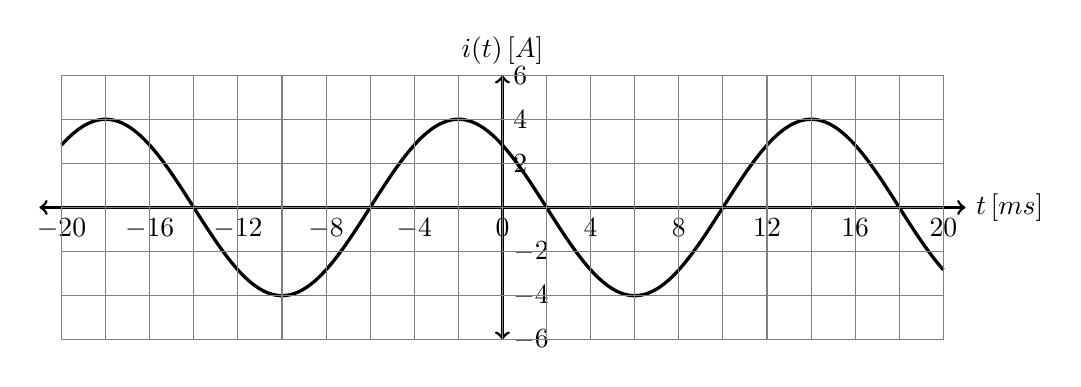
\begin{tikzpicture}[xscale=0.28, yscale=0.28]
    \draw[<->,line width=1pt] (-21,0) -- (21,0) node[right] {$t \, [ms]$};
    \draw[<->,line width=1pt] (0,-6) -- (0,6) node[above] {$i(t) \, [A]$};

    \draw[scale=1,domain=-20:20,variable=\x,black,line width=1.2pt,samples=1000,opacity=1] 
    plot({\x},{4*cos(((3.1415927/8)*\x+(3.1415927/4)) r)});
      
      
    
    \foreach \i in {-20,-16,-12,-8,-4,0,4,8,12,16,20} {
        \draw (\i,0) -- (\i,-0.05) node[below] {$\i$};
    }
    
    \draw (0,6) -- (0.05,6) node[right] {$6$};
    \draw (0,4) -- (0.05,4) node[right] {$4$};
    \draw (0,2) -- (0.05,2) node[right] {$2$};
    \draw (0,-6) -- (0.05,-6) node[right] {$-6$};
    \draw (0,-4) -- (0.05,-4) node[right] {$-4$};
    \draw (0,-2) -- (0.05,-2) node[right] {$-2$};
    
    \draw[step=2cm,color=gray, thin] (-20.01,-6.01) grid (20,6);
    
  \end{tikzpicture}

\end{document}